\documentclass{article}
\usepackage[italian]{babel}
\usepackage{graphicx}
\usepackage{amsmath}
\usepackage{booktabs}
\usepackage{multirow}

\title{Differenza di potenziale e sua misurazione}
\author{Orcam}
\date{}

\begin{document}

\maketitle

% Sezione 1: Potenziale di membrana e gradienti ionici
\section{Potenziale di membrana e gradienti ionici}
\begin{itemize}
\item Differenza ionica intra/extra-cellulare:
  \begin{table}[h]
  \centering
  \begin{tabular}{lcc}
  \toprule
  Ione & Intracellulare (mM) & Extracellulare (mM) \\
  \midrule
  Na\(^+\) & 10 & 120 \\
  K\(^+\) & 140 & 3 \\
  Cl\(^-\) & 3-4 & 120 \\
  Ca\(^{2+}\) & <0.001 & 2 \\
  A\(^-\) & 140 & - \\
  \bottomrule
  \end{tabular}
  \caption{Concentrazioni ioniche a riposo}
  \end{table}

\item Origine del potenziale transmembrana (\(V_m \approx -70 \, \text{mV}\)):
  \begin{itemize}
  \item Permeabilità selettiva ai K\(^+\) (30× > Na\(^+\))
  \item Anioni non diffusibili (proteine)
  \end{itemize}

\begin{figure}[h]
\centering
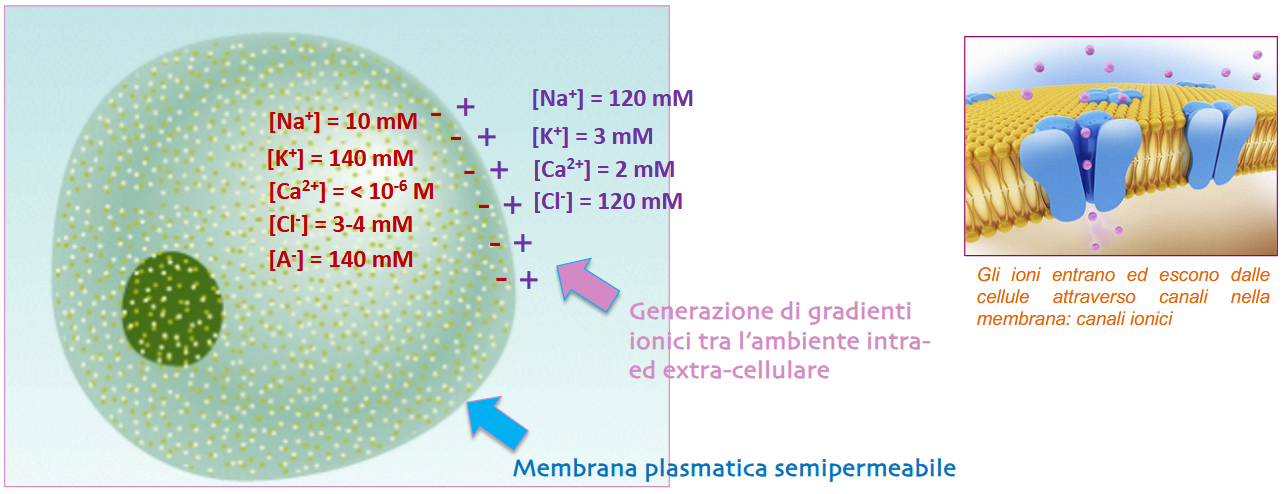
\includegraphics[width=1\textwidth]{Neuroscienze 2024-2025/Modulo I/Immagini Modulo I/Screenshot 2025-06-21 at 17-38-29 6. Differenza di potenziale e sua misurazione .pdf.png}
\caption{Distribuzione ionica e generazione del \(V_m\)}
\label{fig:gradienti}
\end{figure}
\end{itemize}

% Sezione 2: Equilibrio di Donnan
\section{Equilibrio di Donnan (1911)}
\[
[K^+]_1 \cdot [C^-]_1 = [K^+]_2 \cdot [C^-]_2
\]
\begin{itemize}
\item Condizioni:
  \begin{itemize}
  \item Elettroneutralità in ogni compartimento
  \item Presenza di ioni non diffusibili (A\(^-\))
  \end{itemize}
\item \textbf{Non applicabile alle cellule} per:
  \begin{itemize}
  \item Attività della pompa Na\(^+\)/K\(^+\) ATPasi
  \item Impermeabilità a Na\(^+\) e Ca\(^{2+}\)
  \end{itemize}

\begin{figure}[h]
\centering
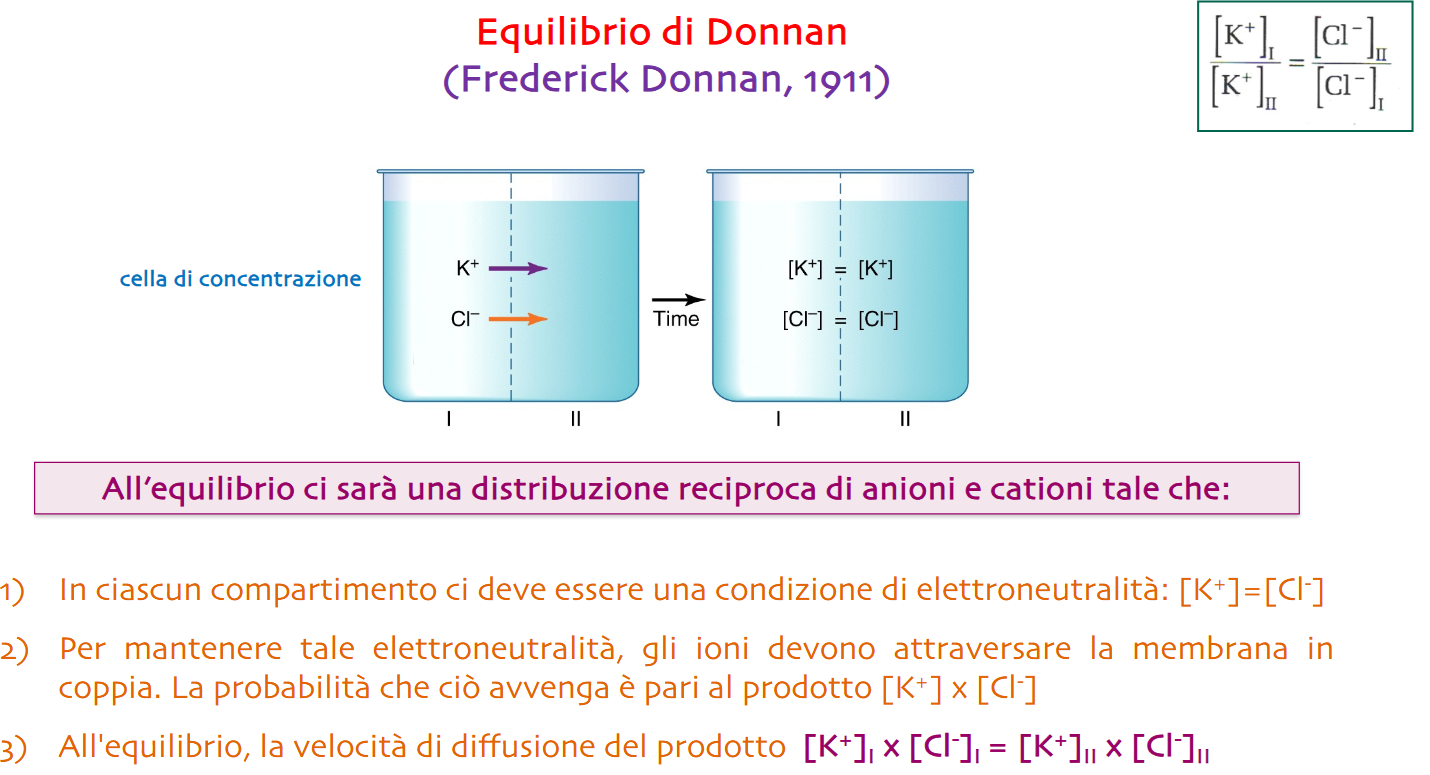
\includegraphics[width=1\textwidth]{Neuroscienze 2024-2025/Modulo I/Immagini Modulo I/Screenshot 2025-06-21 at 17-40-13 6. Differenza di potenziale e sua misurazione .pdf.png}
\caption{Equilibrio di Donnan in sistema semplificato}
\label{fig:donnan}
\end{figure}
\end{itemize}

% Sezione 3: Stato stazionario ionico
\section{Stato stazionario ionico}
\begin{itemize}
\item Mantenuto da:
  \begin{itemize}
  \item Pompa Na\(^+\)/K\(^+\) ATPasi (3 Na\(^+\) out / 2 K\(^+\) in per ATP)
  \item Canali passivi per K\(^+\) e Cl\(^-\)
  \end{itemize}

\item Energia richiesta: 20-50\% del consumo cellulare
\end{itemize}

% Sezione 4: Forza elettromotrice
\section{Forza elettromotrice e gradiente elettrochimico}
\[
\Delta \mu = zF \Delta \psi + RT \ln\left(\frac{[X]_{ext}}{[X]_{int}}\right)
\]
\begin{itemize}
\item \( \Delta \psi \): Differenza di potenziale
\item \( z \): Valenza ionica
\item Movimento ionico determinato da:
  \begin{itemize}
  \item Gradiente chimico
  \item Gradiente elettrico
  \end{itemize}

\begin{figure}[h]
\centering
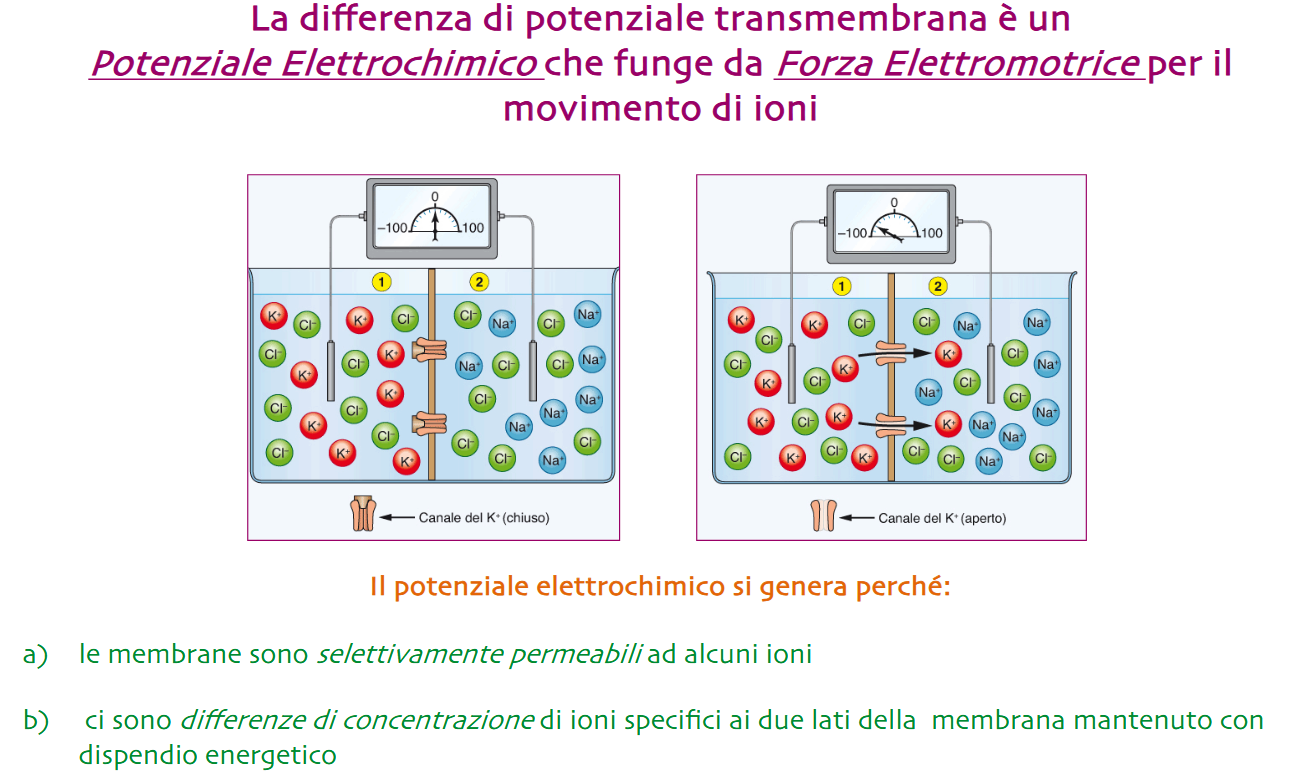
\includegraphics[width=1\textwidth]{Neuroscienze 2024-2025/Modulo I/Immagini Modulo I/Screenshot 2025-06-21 at 17-43-48 6. Differenza di potenziale e sua misurazione .pdf.png}
\caption{Bilancio tra forze chimiche ed elettriche}
\label{fig:forza}
\end{figure}
\end{itemize}

% Sezione 5: Strumentazione
\section{Misurazione del potenziale}
\begin{itemize}
\item Componenti chiave:
  \begin{itemize}
  \item \textbf{Microelettrodo} (Ø ≤1 µm, KCl 3M)
  \item \textbf{Elettrodo di riferimento} (Ag/AgCl)
  \item \textbf{Amplificatore operazionale} (guadagno 10\(^3\)-10\(^5\))
  \end{itemize}

\begin{figure}[h]
\centering
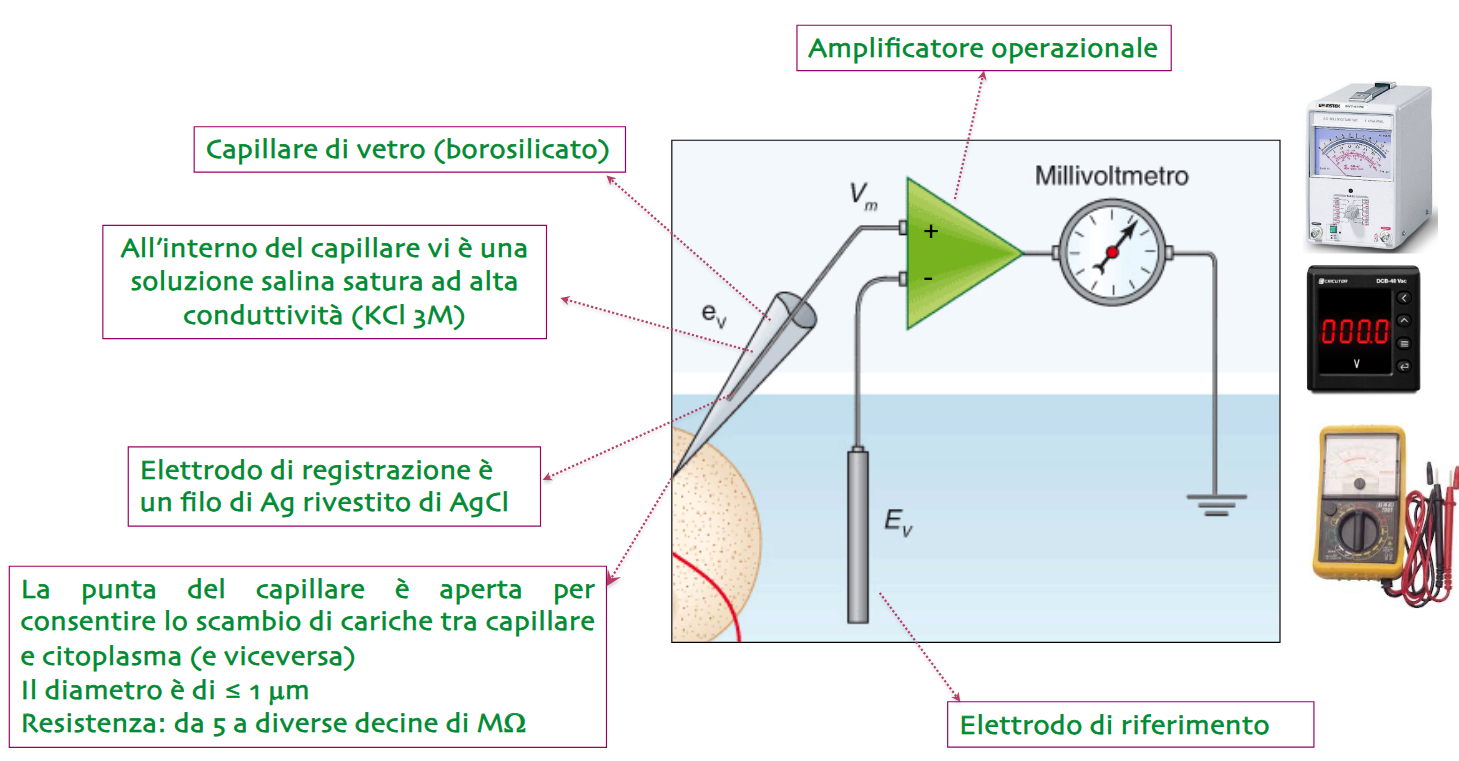
\includegraphics[width=1\textwidth]{Neuroscienze 2024-2025/Modulo I/Immagini Modulo I/Screenshot 2025-06-21 at 17-44-45 6. Differenza di potenziale e sua misurazione .pdf.png}
\caption{Schema apparato di registrazione intracellulare}
\label{fig:amplificatore}
\end{figure}

\item Funzionamento amplificatore:
  \[
  V_{out} = A \cdot (V_+ - V_-)
  \]
  \begin{itemize}
  \item Reiezione modo comune (CMRR > 100 dB)
  \item Alimentazione duale (±15V)
  \end{itemize}
\end{itemize}

% Sezione 6: Ruolo della pompa Na+/K+
\section{Ruolo della pompa Na\(^+\)/K\(^+\) ATPasi}
\begin{itemize}
\item Mantiene:
  \begin{itemize}
  \item Gradienti ionici
  \item \(V_m\) stabile (-70 mV)
  \item Volume cellulare
  \end{itemize}

\begin{figure}[h]
\centering
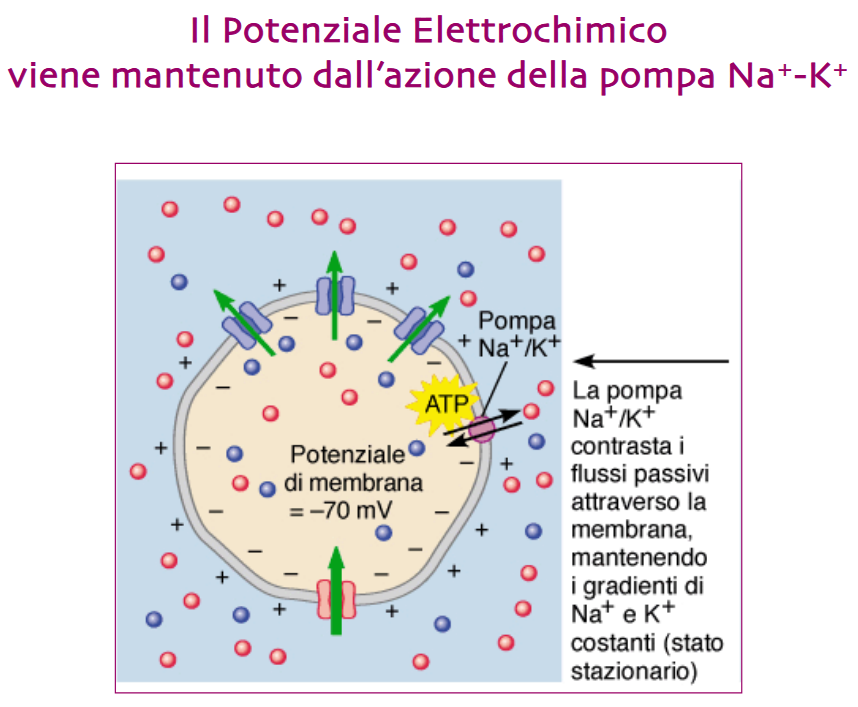
\includegraphics[width=1\textwidth]{Neuroscienze 2024-2025/Modulo I/Immagini Modulo I/Screenshot 2025-06-21 at 17-45-10 6. Differenza di potenziale e sua misurazione .pdf.png}
\caption{Meccanismo della pompa Na\(^+\)/K\(^+\)}
\label{fig:pompa}
\end{figure}
\end{itemize}

\end{document}